% System model of the formulation-4 RL (2026-11-22_formulation_4/baseline_RL/code).
% Standalone: pdflatex system_model.tex  ->  system_model.pdf  (system_model.svg: pdftocairo -svg).
% For a paper: copy the tikzpicture and its styles; needs \usetikzlibrary{arrows.meta,fit,backgrounds,calc}.
% Every block is traced to the code in code_traceability.md (section "System model").
\documentclass[border=6pt]{standalone}
\usepackage{lmodern}
\usepackage[T1]{fontenc}
\usepackage{amsmath,amssymb}
\usepackage{tikz}
\usetikzlibrary{arrows.meta,fit,backgrounds,calc}
\begin{document}
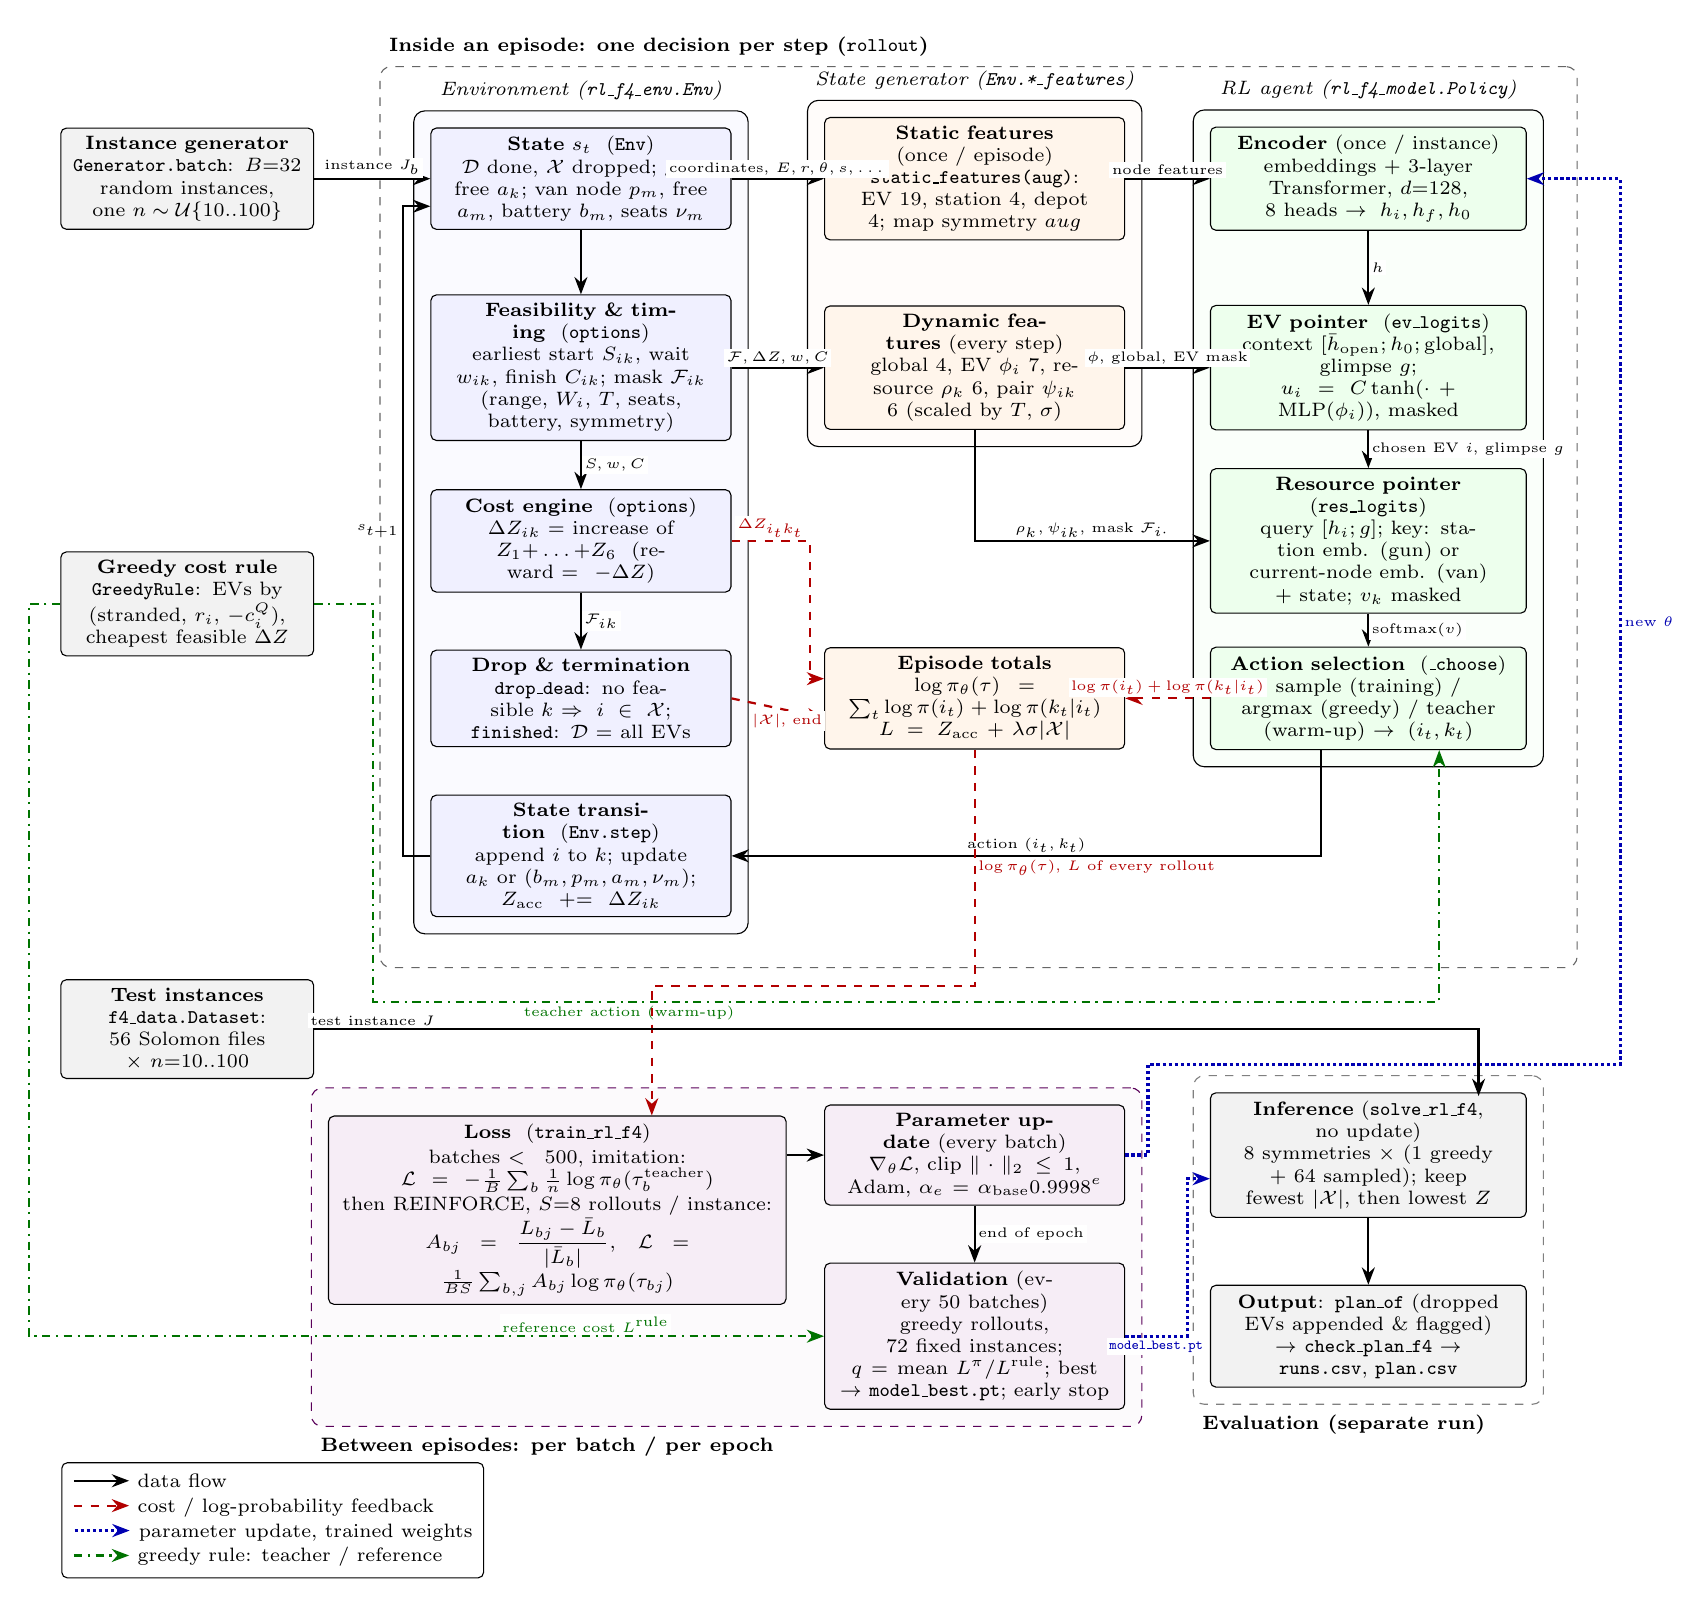
\begin{tikzpicture}[
  font=\scriptsize,
  >={Stealth[length=2.2mm]},
  blk/.style={draw, rounded corners=2pt, align=center, text width=#1, inner sep=3pt, fill=white},
  env/.style={blk=3.6cm, fill=blue!6},
  feat/.style={blk=3.6cm, fill=orange!8},
  agent/.style={blk=3.8cm, fill=green!7},
  upd/.style={blk=#1, fill=violet!7},
  io/.style={blk=#1, fill=gray!10},
  data/.style={->, thick},
  fb/.style={->, thick, red!70!black, dashed},
  par/.style={->, very thick, blue!70!black, densely dotted},
  teach/.style={->, thick, green!45!black, dash dot},
  frame/.style={draw, rounded corners=4pt, inner sep=6pt},
  lab/.style={font=\tiny, fill=white, inner sep=1pt},
]
% ============================================================ inputs (left)
\node[io=3.0cm] (gen)  at (0,12)  {\textbf{Instance generator}\\ \texttt{Generator.batch}: $B{=}32$ random instances, one $n\!\sim\!\mathcal U\{10..100\}$};
\node[io=3.0cm] (rule) at (0,6.6) {\textbf{Greedy cost rule}\\ \texttt{GreedyRule}: EVs by (stranded, $r_i$, $-c^Q_i$), cheapest feasible $\Delta Z$};
\node[io=3.0cm] (test) at (0,1.2) {\textbf{Test instances}\\ \texttt{f4\_data.Dataset}: 56 Solomon files $\times$ $n{=}10..100$};

% ============================================================ environment
\node[env] (state) at (5,12)  {\textbf{State $s_t$} \ (\texttt{Env})\\ $\mathcal D$ done, $\mathcal X$ dropped; gun free $a_k$; van node $p_m$, free $a_m$, battery $b_m$, seats $\nu_m$};
\node[env] (opt)   at (5,9.6) {\textbf{Feasibility \& timing} \ (\texttt{options})\\ earliest start $S_{ik}$, wait $w_{ik}$, finish $C_{ik}$; mask $\mathcal F_{ik}$ (range, $W_i$, $T$, seats, battery, symmetry)};
\node[env] (cost)  at (5,7.4) {\textbf{Cost engine} \ (\texttt{options})\\ $\Delta Z_{ik}$ = increase of $Z_1{+}\dots{+}Z_6$ \ (reward $=-\Delta Z$)};
\node[env] (drop)  at (5,5.4) {\textbf{Drop \& termination}\\ \texttt{drop\_dead}: no feasible $k$ $\Rightarrow i\in\mathcal X$;\ \texttt{finished}: $\mathcal D$ = all EVs};
\node[env] (step)  at (5,3.4) {\textbf{State transition} \ (\texttt{Env.step})\\ append $i$ to $k$; update $a_k$ or $(b_m,p_m,a_m,\nu_m)$; $Z_{\text{acc}}\mathrel{+}=\Delta Z_{ik}$};

% ============================================================ state generator
\node[feat] (sfeat) at (10,12)  {\textbf{Static features} (once / episode)\\ \texttt{static\_features(aug)}: EV 19, station 4, depot 4; map symmetry $aug$};
\node[feat] (dfeat) at (10,9.6) {\textbf{Dynamic features} (every step)\\ global 4, EV $\phi_i$ 7, resource $\rho_k$ 6, pair $\psi_{ik}$ 6 (scaled by $T$, $\sigma$)};
\node[feat] (acc)   at (10,5.4) {\textbf{Episode totals}\\ $\log\pi_\theta(\tau)=\sum_t\log\pi(i_t)+\log\pi(k_t|i_t)$\\ $L=Z_{\text{acc}}+\lambda\sigma|\mathcal X|$};

% ============================================================ agent
\node[agent] (enc)    at (15,12)  {\textbf{Encoder} (once / instance)\\ embeddings + 3-layer Transformer, $d{=}128$, 8 heads $\to h_i,h_f,h_0$};
\node[agent] (evdec)  at (15,9.6) {\textbf{EV pointer} \ (\texttt{ev\_logits})\\ context $[\bar h_{\text{open}};h_0;\text{global}]$, glimpse $g$;\\ $u_i=C\tanh(\cdot+\mathrm{MLP}(\phi_i))$, masked};
\node[agent] (resdec) at (15,7.4) {\textbf{Resource pointer} \ (\texttt{res\_logits})\\ query $[h_i;g]$; key: station emb. (gun) or current-node emb. (van) + state;\ $v_k$ masked};
\node[agent] (sel)    at (15,5.4) {\textbf{Action selection} \ (\texttt{\_choose})\\ sample (training) / argmax (greedy) / teacher (warm-up) $\to(i_t,k_t)$};

% ============================================================ between episodes
\node[upd=5.6cm] (loss) at (4.7,-1.1) {\textbf{Loss} \ (\texttt{train\_rl\_f4})\\[1pt]
   batches $<500$, imitation: $\mathcal L=-\frac1B\sum_b\frac1n\log\pi_\theta(\tau^{\text{teacher}}_b)$\\[1pt]
   then REINFORCE, $S{=}8$ rollouts / instance:\\ $A_{bj}=\dfrac{L_{bj}-\bar L_b}{|\bar L_b|}$,\quad $\mathcal L=\frac{1}{BS}\sum_{b,j}A_{bj}\log\pi_\theta(\tau_{bj})$};
\node[upd=3.6cm] (adam) at (10,-0.4) {\textbf{Parameter update} (every batch)\\ $\nabla_\theta\mathcal L$, clip $\|\cdot\|_2\le1$, Adam, $\alpha_e=\alpha_{\text{base}}0.9998^{e}$};
\node[upd=3.6cm] (val)  at (10,-2.7) {\textbf{Validation} (every 50 batches)\\ greedy rollouts, 72 fixed instances; $q=\text{mean }L^\pi/L^{\text{rule}}$; best $\to$ \texttt{model\_best.pt}; early stop};

% ============================================================ inference
\node[io=3.8cm] (inf) at (15,-0.4) {\textbf{Inference} (\texttt{solve\_rl\_f4}, no update)\\ 8 symmetries $\times$ (1 greedy + 64 sampled); keep fewest $|\mathcal X|$, then lowest $Z$};
\node[io=3.8cm] (out) at (15,-2.7) {\textbf{Output}: \texttt{plan\_of} (dropped EVs appended \& flagged) $\to$ \texttt{check\_plan\_f4} $\to$ \texttt{runs.csv}, \texttt{plan.csv}};

% ============================================================ frames
\begin{scope}[on background layer]
  \node[frame, fill=blue!2, fit=(state)(step), label={[font=\scriptsize\itshape]above:Environment (\texttt{rl\_f4\_env.Env})}] (fenv) {};
  \node[frame, fill=orange!2, fit=(sfeat)(dfeat), label={[font=\scriptsize\itshape]above:State generator (\texttt{Env.*\_features})}] (ffeat) {};
  \node[frame, fill=green!2, fit=(enc)(sel), label={[font=\scriptsize\itshape]above:RL agent (\texttt{rl\_f4\_model.Policy})}] (fag) {};
  \node[frame, draw=black!60, dashed, inner sep=12pt, fit=(fenv)(fag)(ffeat)(acc)] (fep) {};
  \node[font=\scriptsize\bfseries, anchor=south west] at (fep.north west) {Inside an episode: one decision per step (\texttt{rollout})};
  \node[frame, draw=violet!70!black, dashed, fill=violet!2, fit=(loss)(adam)(val)] (fup) {};
  \node[font=\scriptsize\bfseries, anchor=north west] at (fup.south west) {Between episodes: per batch / per epoch};
  \node[frame, draw=black!50, dashed, fit=(inf)(out)] (finf) {};
  \node[font=\scriptsize\bfseries, anchor=north west] at (finf.south west) {Evaluation (separate run)};
\end{scope}

% ============================================================ arrows inside the episode
\draw[data] (gen.east) -- node[lab, above]{instance $J_b$} ($(state.west)+(0,0)$);
\draw[data] (state) -- (opt);
\draw[data] (opt) -- node[lab, right]{$S,w,C$} (cost);
\draw[data] (cost) -- node[lab, right]{$\mathcal F_{ik}$} (drop);
\draw[data] (state.east) -- node[lab, above]{coordinates, $E,r,\theta,s,\dots$} (sfeat.west);
\draw[data] (sfeat.east) -- node[lab, above]{node features} (enc.west);
\draw[data] (opt.east) -- node[lab, above]{$\mathcal F,\Delta Z,w,C$} (dfeat.west);
\draw[data] (dfeat.east) -- node[lab, above]{$\phi$, global, EV mask} (evdec.west);
\draw[data] (dfeat.south) |- node[lab, above, pos=0.75]{$\rho_k,\psi_{ik}$, mask $\mathcal F_{i\cdot}$} (resdec.west);
\draw[data] (enc) -- node[lab, right]{$h$} (evdec);
\draw[data] (evdec) -- node[lab, right]{chosen EV $i$, glimpse $g$} (resdec);
\draw[data] (resdec) -- node[lab, right]{$\mathrm{softmax}(v)$} (sel);
\draw[data] ($(sel.south)+(-0.6,0)$) |- node[lab, above, pos=0.75]{action $(i_t,k_t)$} (step.east);
\draw[data] (step.west) -- ++(-0.35,0) |- node[lab, left, pos=0.25]{$s_{t+1}$} ($(state.west)+(0,-0.35)$);
\draw[fb] (cost.east) -- node[lab, above]{$\Delta Z_{i_tk_t}$} ++(1.0,0) |- ($(acc.west)+(0,0.25)$);
\draw[fb] (drop.east) -- node[lab, below, pos=0.6]{$|\mathcal X|$, end} ($(acc.west)+(0,-0.25)$);
\draw[fb] (sel.west) -- node[lab, above]{$\log\pi(i_t)+\log\pi(k_t|i_t)$} (acc.east);
\draw[teach] (rule.east) -- ++(0.75,0) |- node[lab, below, pos=0.62]{teacher action (warm-up)} ($(sel.south)+(0.9,-3.2)$) -- ($(sel.south)+(0.9,0)$);

% ============================================================ arrows between episodes
\draw[fb] (acc.south) -- node[lab, right, pos=0.5]{$\log\pi_\theta(\tau)$, $L$ of every rollout} ++(0,-3.0) -| ($(loss.north)+(1.2,0)$);
\draw[data] (loss.east|-adam.west) -- (adam.west);
\draw[par] (adam.east) -- (12.2,-0.4) -- (12.2,0.75) -- (18.2,0.75) -- node[lab, right, pos=0.5]{new $\theta$} (18.2,12) -- (enc.east);
\draw[data] (adam) -- node[lab, right]{end of epoch} (val);
\draw[teach] (rule.west) -- ++(-0.4,0) |- node[lab, above, pos=0.85]{reference cost $L^{\text{rule}}$} (val.west);

% ============================================================ inference
\draw[par] (val.east) -- node[lab, below]{\texttt{model\_best.pt}} (12.7,-2.7) |- ($(inf.west)+(0,-0.3)$);
\draw[data] (test.east) -- node[lab, above, pos=0.05]{test instance $J$} (16.4,1.2) -- (16.4,0.35);
\draw[data] (inf) -- (out);

% ============================================================ legend
\node[anchor=north west, align=left, draw, rounded corners=2pt, fill=white, inner sep=4pt] at (-1.6,-4.3) {%
  \tikz{\draw[data] (0,0)--(0.7,0);} data flow\\[1pt]
  \tikz{\draw[fb] (0,0)--(0.7,0);} cost / log-probability feedback\\[1pt]
  \tikz{\draw[par] (0,0)--(0.7,0);} parameter update, trained weights\\[1pt]
  \tikz{\draw[teach] (0,0)--(0.7,0);} greedy rule: teacher / reference};
\end{tikzpicture}
\end{document}
